\documentclass[addpoints, 12pt]{exam}
\usepackage[export]{adjustbox}
\usepackage{amsmath}
\usepackage{amsthm}
\usepackage{amssymb}
\usepackage{amsfonts}
\usepackage{blox}
\usepackage{bm}
\usepackage{caption}
\usepackage{breqn}
\usepackage{enumitem}
\usepackage{epsfig}
\usepackage{epstopdf}
\usepackage[letterpaper, top=1.0in, bottom=1.0in, left=0.75in, right=0.75in]{geometry}
\usepackage{graphics} % for pdf, bitmapped graphics files
\usepackage{graphicx}
\usepackage{listings}
\usepackage{nicefrac}
\usepackage{siunitx}
\sisetup{per-mode=symbol}
\usepackage{subcaption}
% \captionsetup{justification=raggedright,singlelinecheck=false}
\usepackage{tikz}
\usepackage{tkz-euclide}
% \usepackage{units}
\usepackage{ctable}
\usetikzlibrary{matrix, arrows}
\usepackage{wrapfig}

% \usepackage{nicematrix}
% \NiceMatrixOptions{code-for-first-row = \scriptstyle}

% \NiceMatrixOptions{code-for-first-row=\color{red},
%                    code-for-first-col=\color{blue},
%                    code-for-last-row=\color{green},
%                    code-for-last-col=\color{magenta}}



\makeatletter
\newcommand{\rmnum}[1]{\romannumeral #1}
\newcommand{\Rmnum}[1]{\expandafter\@slowromancap\romannumeral #1@}
\makeatother


\newcommand*\circled[1]{\tikz[baseline=(char.base)]{
            \node[shape=circle,draw,inner sep=2pt] (char) {#1};}}

\newcommand{\bmat}[1]{\begin{bmatrix}#1\end{bmatrix}}
\newcommand{\dd}{\operatorname{d}\!}
\newcommand{\norm}[2]{\|{#1}\|_{{}_{#2}}}
\newcommand{\abs}[1]{\left|{#1}\right|}
\newcommand{\mc}[1]{\mathcal{#1}}
\newcommand{\pd}[2]{\frac{\partial #1}{\partial #2}}
\newcommand{\pdd}[2]{\frac{\partial^2 #1}{\partial #2^2}}
\newcommand{\mbf}[1]{\boldsymbol{\mathbf{#1}}}

\pagestyle{headandfoot}
\firstpageheader{FE: Dynamics and Kinematics}{Quiz}{Mar 25, 2024}
\firstpagefooter{}{}{}
\runningheader{FE: Dynamics and Kinematics}{Quiz}
{Mar 25, 2024}
\firstpageheadrule
\runningheadrule
\runningfooter{}{Page \thepage\ of \numpages}{}
% \runningfootrule



\begin{document}

\renewcommand{\arraystretch}{1.25}

\begin{center}
% \fbox{\fbox{\parbox{5.5in}{\centering
% Answer the questions in the spaces provided on the
% question sheets. If you run out of room for an answer,
% continue on the back of the page.}}}
% \end{center}

{\Large FE: Dynamics and Kinematics \\[0ex]
Spring $2024$ | Quiz} \\[2ex]
{\large Aykut C. Satici}
\end{center}

% \vspace{0.0in}
% \makebox[0.9\textwidth]{Name:\enspace\hrulefill}

% \vspace{0.8in}
% \noindent \textit{Note that the questions are not weighted equally. Budget your
% time accordingly and do not work too long on any one problem. If you feel that a
% question is ambiguous, give your reasons and state your assumptions.}

% \vspace{0.1in}
% \begin{minipage}{0.4\textwidth}
%     \noindent \textbf{Laplace Transform Pairs}
% 
%     \begin{adjustbox}{width=1.0\textwidth}
% %     \resizebox{\textwidth}{!}{
%     \begin{tabular}{ccc}
%     $f(t)$ & $\mc{L}\{f(t)\}$ & Poles  \\
%     \hline 
%     $\delta(t)$ & $1$ & \\
%     $u_s(t)$ & $\frac{1}{s}$ & $p = 0$\\
%     $t u_s(t)$ & $\frac{1}{s^2}$ & $p=0,0$\\
%     $t^n u_s(t)$ & $\frac{n!}{s^{n+1}}$ & $p = \underbrace{0, \ldots, 0}_{n+1
%             \text{ times}}$\\
%     $e^{rt}u_s(t)$ & $\frac{1}{s-r}$ & $p = r$\\
%     $t^n e^{rt} u_s(t)$ & $\frac{n!}{(s-r)^{n+1}}$ & $p = \underbrace{r, \ldots, r}_{n+1
%             \text{ times}}$\\
%     $\sin{(\omega t)} u_s(t)$ & $\frac{\omega}{s^2+\omega^2}$ & $p = \pm j \omega$\\
%     $\cos{(\omega t)} u_s(t)$ & $\frac{s}{s^2+\omega^2}$ & $p = \pm j
%     \omega $\\
%     $e^{\sigma t}\sin{(\omega t)} u_s(t)$ & $\frac{\omega}{(s-\sigma)^2 +
%     \omega^2}$ & $p=\sigma \pm j \omega$ \\
%     $e^{\sigma t}\cos{(\omega t)} u_s(t)$ & $\frac{s-\sigma}{(s-\sigma)^2 +
%     \omega^2}$ & $p = \sigma \pm j\omega$ \\
%     $t \sin{(\omega t)} u_s(t)$ & $\frac{2\omega s}{\left(s^2 +
%     \omega^2\right)^2}$ & $p = \pm j\omega, \pm j\omega$ \\
%     $t \cos{(\omega t)} u_s(t)$ & $\frac{s^2-\omega^2}{\left(s^2 +
%     \omega^2\right)^2}$ & $p = \pm j\omega, \pm j\omega$\\
%     \hline 
%     \end{tabular}
% % }
%     \end{adjustbox}\\[2ex]
% 
%     \noindent \textbf{Laplace Transform Properties}
%     %  
%     \footnotesize{
%     \begin{align*}
%     \mc{L}{\left\{ \int_0^t x(\tau) d\tau \right\}} &= \nicefrac{1}{s}X(s) \\
%     \mc{L}{\left\{ \frac{d}{dt}f(t) \right\}} &= s F(s) - f(0) \\
%     \mc{L}{\left\{ e^{at}f(t) \right\}} &= F(s-a) \\
%     \mc{L}{\left\{ tf(t) \right\}} &= -\nicefrac{d}{ds}F(s) \\
% %     \mc{L}{\left\{ \int_0^t f(\tau)d\tau \}\right\}} &= \nicefrac{1}{s}F(s)
%     \end{align*}
% }
% \normalsize
% \vspace{-2mm}
%     %
%     \noindent \textbf{Quadratic Formula}
%     %
%     \footnotesize{
%     \[ c + bx + ax^2 = 0 \Rightarrow x = \frac{-b \pm \sqrt{b^2- 4ac}}{2a} \]}
% 
%     \normalsize{
%     \noindent \textbf{Time-Domain Specifications}
% }\\[0.5ex] 
% \footnotesize
% 
%     \begin{tabular}{ll}
%         Frac. Overshoot: & $M_p \triangleq
% \frac{c(t_p)-c(\infty)}{c(\infty)}$ \\
%         Settling time: & $\abs{c(t) - R_0} \leq \nicefrac{2}{100}R_0$
%     \end{tabular}\\[2ex]
% 
%     \small
%     \noindent \textbf{Elem. Symmetric Polynomials}
%     \footnotesize
%     \begin{align*}
%         &e_k(p_1,\ldots,p_n) = \sum_{1 \leq j_1 < \ldots < j_k \leq n} p_{j_1} \cdots
%     p_{j_k} \\
% %          &\prod_{j=1}^n (s-p_j) = s^n - e_1s^{n-1} + e_2s^{n-2} \\ 
% %          &\hspace{7mm} - \ldots + (-1)^{n-1}e_{n-1}s^1+ (-1)^ne_n.
%         &\prod_{j=1}^n (s-p_j) = \sum_{j=0}^n (-1)^{n-j}e_{n-j}s^j.
%     \end{align*} 
% 
% \end{minipage}
% %
% \begin{minipage}{0.6\textwidth}
%    \normalsize 
%    %  \centering 
%     \noindent \textbf{Block Diagrams}\\[-2ex]
%     % 
%     \begin{small}
%     \begin{tikzpicture}[scale=0.75]
%         \bXInput{A}
%         \begin{footnotesize}
%         \bXComp{B}{A}
%         \end{footnotesize}
%         \bXLink[$r$]{A}{B}
%         \bXBloc[2]{C}{$G_c$}{B}
%         \bXLink[$e$]{B}{C}
% %         \begin{small}
%         \begin{footnotesize}
%         \bXCompa{D}{C}
%         \end{footnotesize}
% %         \end{small}
%         \bXBloc[2]{E}{$G_m$}{D}
%         \bXOutput{I}{E}\bXLinkName[.6]{I}{$c$}
%         \bXLink{C}{D}
%         \bXLink{D}{E}
%         \bXLink{E}{I}
%         \bXReturn{E-I}{B}{}
%         \bXBranchy[-4]{D}{H}
%         \bXLink[$d$]{H}{D}
%     \end{tikzpicture}
%     \end{small}
%     %
%     \footnotesize{
%     \begin{align*}
%     C(s) &= \frac{G_c(s)G_m(s)}{1 + G_c(s)G_m(s)}R(s) -
%     \frac{G_m(s)}{1+G_c(s)G_m(s)}D(s) \\[1ex]
%     E(s) &= R(s) - C(s) \\
%          &= \frac{1}{1+G_c(s)G_m(s)}R(s) + \frac{G_m(s)}{1+G_c(s)G_m(s)}D(s)
%     \end{align*}
%     }
% 
%     \noindent \footnotesize{\textbf{Step Response of a $2^{\text{nd}}$-Order
%     System}}\\[-2ex]
%     
%     \begin{center}
%     \begin{small}
%     \begin{tikzpicture}
%     \bXInput{A}
%     \bXBranchx[2]{A}{G}
%     \begin{footnotesize}
%     \bXComp{B}{G}
%     \end{footnotesize}
%     \bXLink[$R=\nicefrac{R_0}{s}$]{A}{B}
%     \bXBloc[2]{C}{$G = \frac{\omega_n^2}{s^2+2\zeta\omega_ns}$}{B}
%     \bXLink[$e$]{B}{C}
%     \bXOutput{E}{C}
%     \bXLink[$c$]{C}{E}
%     \bXReturn{C-E}{B}{}
%     \end{tikzpicture}
%     \end{small}
%     \end{center}
%     % 
%     \begin{align*}
%     \frac{C(s)}{R(s)} &= \frac{G(s)}{1+G(s)} = \frac{\omega_n^2}{s^2 +
%             2\zeta\omega_ns + \omega_n^2} \\
%     C(s) &= \frac{\omega_n^2}{s^2 + 2\zeta\omega_ns + \omega_n^2}\frac{R_0}{s}
%     \\
%     c(t) &= R_0 - R_0e^{-\zeta \omega_n t}\left( \cos{(\omega_d t)} +
%             \frac{\zeta}{\sqrt{1-\zeta^2}}\sin{(\omega_d t)}  \right) \\
%     \omega_d &\triangleq \omega_n \sqrt{1 - \zeta^2}
%     \end{align*}
% 
%     \begin{center}
%     \begin{tabular}{ccc}
%         Peak time & Max. overshoot & Settling time ($\zeta \leq 0.3$)\\ \hline
%         $t_p = \nicefrac{\pi}{\omega_d}$ & $M_p = e^{-\zeta \omega_n t_p}$ & 
%         $-\nicefrac{1}{\zeta \omega_n}\ln{\left(\nicefrac{2}{100}\sqrt{1-\zeta^2}\right)}$
%     \end{tabular}
%     \end{center}
%     As $\zeta \to 1$, above setting time formula is not useful; instead use
%     \[ t_s \triangleq \nicefrac{4}{\zeta\omega_n}. \]
% 
%     \renewcommand{\arraystretch}{1}
% 
%     \begin{minipage}{0.3\textwidth}
% 
%     \footnotesize
%     \begin{center}
%     \begin{align*}
%         \zeta &= \sqrt{\frac{\ln^2{(M_p)}}{\pi^2 + \ln^2{(M_p)}}} \\
%         M_p &= \exp{\left(-\frac{\zeta}{\sqrt{1-\zeta^2}}\pi\right)}
%     \end{align*}
%     \end{center}
%     \end{minipage}
%     \begin{minipage}{0.7\textwidth}
%     \begin{center}
%         \begin{tabular}{ccc}
%                 $M_p$ & $\zeta$ & $\sqrt{1-\zeta^2}$ \\ \hline
%             $0.05$ & $0.690$ & $0.724$ \\
%             $0.1$ & $0.591$ & $0.807$ \\
% %             $0.15$ & $0.517$ & $0.856$ \\
% %             $0.163$ & $0.5$ & $0.866$ \\
%             $0.2$ & $0.456$ & $0.890$ \\
% %             $0.223$ & $0.431$ & $1.108$ \\
%             $0.25$ & $0.403$ & $0.915$ \\
%             $0.3$ & $0.358$ & $0.934$
%         \end{tabular}
%     \end{center}
%     \end{minipage}
% \end{minipage}

\renewcommand{\arraystretch}{1.25}



% \bracketedpoints

% \newpage

\begin{questions}


\begin{minipage}{0.5\textwidth}
\question(\textit{Particle Kinematics})
A rocket is fired vertically upward from a launching pad at $B$, and its flight
is tracked by the radar at point A. Find the magnitude of the velocity of the 
rocket when $\theta = 45^\circ$ if $\dot{\theta} = \nicefrac{1}{10}\;
\unit[per-mode=symbol]{\radian\per\second}$. \\[0.5ex]

\begin{minipage}{0.3\textwidth}
    \begin{center}
    \begin{itemize}
        \setlength\itemsep{-0.4em}
        \item[a.] $36 \; \unit[per-mode=symbol]{\meter\per\second}$
        \item[b.] $180 \; \unit[per-mode=symbol]{\meter\per\second}$
    \end{itemize}
    \end{center}
\end{minipage}
\begin{minipage}{0.3\textwidth}
    \begin{center}
    \begin{itemize}
        \setlength\itemsep{-0.4em}
        \item[c.] $90 \; \unit[per-mode=symbol]{\meter\per\second}$
        \item[\circled{d.}] $360 \; \unit[per-mode=symbol]{\meter\per\second}$
    \end{itemize}
    \end{center}
\end{minipage}

\end{minipage}
%
% \begin{figure}[h]
\begin{minipage}{0.5\textwidth}
    \centering
    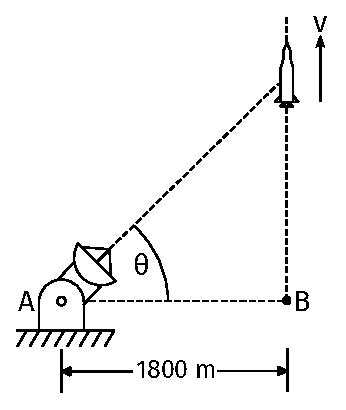
\includegraphics[width=0.55\textwidth,valign=c]{./figures/question1.eps}
%     \captionsetup{labelformat=empty}
%     \caption{\scriptsize DC motor drawing and schematic}
%     \label{fig:gear_system}
\end{minipage}
% \end{wrapfigure}

\begin{minipage}{0.5\textwidth}
\question(\textit{Rigid-Body Kinematics})
The block $B$ is constrained to move along a horizontal rectilinear path with a 
constant acceleration of $2\; \unit{\meter\per\second\squared}$ to the right. 
The slender rod, $R$, of length $2\; \unit{\meter}$ is pinned to $B$ at $O$ and 
can swing freely in the vertical plane. At the instant when $\theta = 0^\circ$ 
(rod is vertical), the angular velocity of the rod is zero but its angular 
acceleration is $2.5 \; \unit{\meter\per\second\squared}$ clockwise. Find the 
acceleration of the midpoint $G$ of the rod at this instant $(\theta =
0^\circ)$. \\[0.5ex]

\begin{minipage}{0.45\textwidth}
    \begin{center}
    \begin{itemize}
        \setlength\itemsep{-0.4em}
        \item[a.] $3.0 \; \unit{\meter\per\second} \; \leftarrow$
        \item[b.] $0.5 \; \unit{\meter\per\second} \; \rightarrow$
    \end{itemize}
    \end{center}
\end{minipage}
\begin{minipage}{0.45\textwidth}
    \begin{center}
    \begin{itemize}
        \setlength\itemsep{-0.4em}
        \item[\circled{c.}] $0.5 \; \unit{\meter\per\second} \; \leftarrow$
        \item[d.] $2.5 \; \unit{\meter\per\second} \; \rightarrow$
    \end{itemize}
    \end{center}
\end{minipage}

\end{minipage}
%
% \begin{figure}[h]
\begin{minipage}{0.5\textwidth}
    \centering
    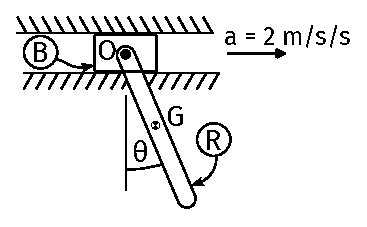
\includegraphics[width=0.8\textwidth,valign=c]{./figures/question2.eps}
%     \captionsetup{labelformat=empty}
%     \caption{\scriptsize DC motor drawing and schematic}
%     \label{fig:gear_system}
\end{minipage}
% \end{wrapfigure}


\begin{minipage}{0.5\textwidth}
\question(\textit{Rigid-Body Kinematics})
The rod $R$ rotates in the vertical plane about a fixed axis through the point 
$O$ with a constant counterclockwise angular velocity of $5 \;
\unit{\radian\per\second}$. A collar $B$ of mass $2 \; \unit{\kilo\gram}$ slides
down the rod (toward $O$) so that the distance between $B$ and $O$ decreases at
the constant rate of $1 \; \unit{\meter\per\second}$. At the instaht when
$\theta = 30^\circ$ and $r = 400 \; \unit{\milli\meter}$, determine the 
magnitude of the applied force $P$. The coefficient of kinetic friction between 
$B$ and $R$ is $\nicefrac{1}{10}$. \\[0.5ex]

\begin{minipage}{0.45\textwidth}
    \begin{center}
    \begin{itemize}
        \setlength\itemsep{-0.4em}
        \item[\circled{a.}] $9.9 \; \unit{\newton}$
        \item[b.] $11.9 \; \unit{\newton}$
    \end{itemize}
    \end{center}
\end{minipage}
\begin{minipage}{0.45\textwidth}
    \begin{center}
    \begin{itemize}
        \setlength\itemsep{-0.4em}
        \item[c.] $10.5 \; \unit{\newton}$
        \item[d.] $0.3 \; \unit{\newton}$
    \end{itemize}
    \end{center}
\end{minipage}

\end{minipage}
%
% \begin{figure}[h]
\begin{minipage}{0.5\textwidth}
    \centering
    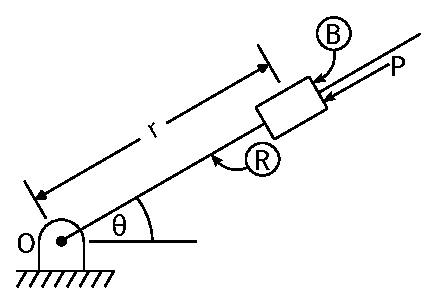
\includegraphics[width=0.8\textwidth,valign=c]{./figures/question3.eps}
%     \captionsetup{labelformat=empty}
%     \caption{\scriptsize DC motor drawing and schematic}
%     \label{fig:gear_system}
\end{minipage}
% \end{wrapfigure}



\begin{minipage}{0.5\textwidth}
\question(\textit{Work-Energy})
A block of mass $2 \; \unit{\kilo\gram}$ is pressed against a linear spring of 
constant $k = 200 \; \unit{\newton\per\meter}$ through a distance $\Delta$ on a 
horizontal surface. When the block is released at $A$, it travels along the 
straight horizontal path $ADB$ and traverses point $B$ with a velocity of $1 \;
\unit{\meter\per\second}$. If the coefficient of kinetic friction between the 
block and the floor is $\nicefrac{2}{10}$, find $\Delta$. \\[0.5ex]

\begin{minipage}{0.45\textwidth}
    \begin{center}
    \begin{itemize}
        \setlength\itemsep{-0.4em}
        \item[a.] $0.22 \; \unit{\meter}$
        \item[b.] $0.12 \; \unit{\meter}$
    \end{itemize}
    \end{center}
\end{minipage}
\begin{minipage}{0.45\textwidth}
    \begin{center}
    \begin{itemize}
        \setlength\itemsep{-0.4em}
        \item[\circled{c.}] $0.26 \; \unit{\meter}$
        \item[d.] $0.08 \; \unit{\meter}$
    \end{itemize}
    \end{center}
\end{minipage}

\end{minipage}
%
% \begin{figure}[h]
\begin{minipage}{0.5\textwidth}
    \centering
    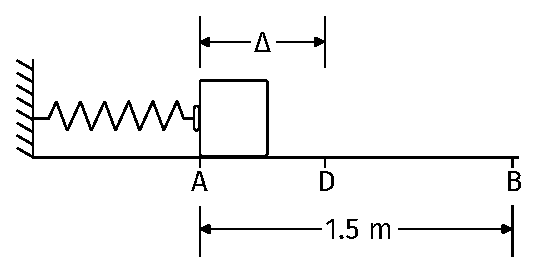
\includegraphics[width=0.8\textwidth,valign=c]{./figures/question4.eps}
%     \captionsetup{labelformat=empty}
%     \caption{\scriptsize DC motor drawing and schematic}
%     \label{fig:gear_system}
\end{minipage}
% \end{wrapfigure}



\begin{minipage}{0.5\textwidth}
\question(\textit{Moment of Inertia})
Two identical rods, each of mass $4 \; \unit{\kilo\gram}$ and length $3 \;
\unit{\meter}$, are rigidly connected as shown in the figure. Determine the
moment of inertia of the rigid assembly about an axis through the point $A$ and 
perpendicular to the plane of the paper. \\[0.5ex]

\begin{minipage}{0.45\textwidth}
    \begin{center}
    \begin{itemize}
        \setlength\itemsep{-0.4em}
        \item[a.] $19 \; \unit{\kilo\gram\,\meter^2}$
        \item[\circled{b.}] $23 \; \unit{\kilo\gram\,\meter^2}$
    \end{itemize}
    \end{center}
\end{minipage}
\begin{minipage}{0.45\textwidth}
    \begin{center}
    \begin{itemize}
        \setlength\itemsep{-0.4em}
        \item[c.] $18 \; \unit{\kilo\gram\,\meter^2}$
        \item[d.] $15 \; \unit{\kilo\gram\,\meter^2}$
    \end{itemize}
    \end{center}
\end{minipage}

\end{minipage}
%
% \begin{figure}[h]
\begin{minipage}{0.5\textwidth}
    \centering
    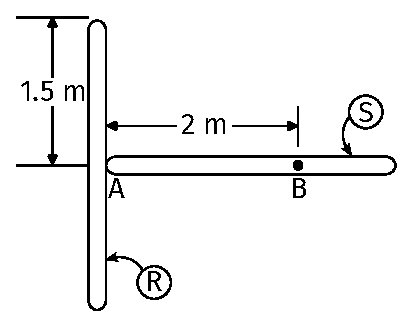
\includegraphics[width=0.6\textwidth,valign=c]{./figures/question5.eps}
%     \captionsetup{labelformat=empty}
%     \caption{\scriptsize DC motor drawing and schematic}
%     \label{fig:gear_system}
\end{minipage}
% \end{wrapfigure}


\begin{minipage}{0.5\textwidth}
\question(\textit{Dynamics})
A homogeneous cylinder rolls without slipping on a horizontal floor under the 
influence of a force $P = 6 \; \unit{\newton}$ and a torque $T = 0.5 \; 
\unit{\newton\,\meter}$. The cylinder has radius $1 \; \unit{\meter}$ and mass 
$2 \; \unit{\kilo\gram}$. If the cylinder started from rest, what is its angular
velocity after $10 \; \unit{\second}$? \\[0.5ex]

\begin{minipage}{0.45\textwidth}
    \begin{center}
    \begin{itemize}
        \setlength\itemsep{-0.4em}
        \item[\circled{a.}] $8.3 \; \unit{\radian\per\second}$
        \item[b.] $6.8 \; \unit{\radian\per\second}$
    \end{itemize}
    \end{center}
\end{minipage}
\begin{minipage}{0.45\textwidth}
    \begin{center}
    \begin{itemize}
        \setlength\itemsep{-0.4em}
        \item[c.] $1.7 \; \unit{\radian\per\second}$
        \item[d.] $0.68 \; \unit{\radian\per\second}$
    \end{itemize}
    \end{center}
\end{minipage}

\end{minipage}
%
% \begin{figure}[h]
\begin{minipage}{0.5\textwidth}
    \centering
    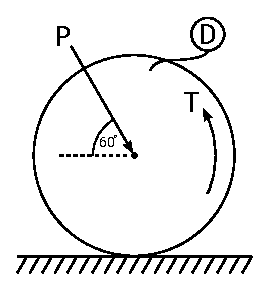
\includegraphics[width=0.5\textwidth,valign=c]{./figures/question6.eps}
%     \captionsetup{labelformat=empty}
%     \caption{\scriptsize DC motor drawing and schematic}
%     \label{fig:gear_system}
\end{minipage}
% \end{wrapfigure}


\begin{minipage}{0.5\textwidth}
\question(\textit{Work-Energy})
A solid homogeneous cylinder is released from rest in the position shown and 
rolls without slip on a horizontal floor. The cylinder has a mass of $12 \; 
\unit{\kilo\gram}$. The spring constant is $2 \; \unit{\newton\per\meter}$, and 
the unstretched length of the spring is $3 \; \unit{\meter}$. What is the 
angular velocity of the cylinder when its center is directly below the point
$O$? \\[0.5ex]

\begin{minipage}{0.45\textwidth}
    \begin{center}
    \begin{itemize}
        \setlength\itemsep{-0.4em}
        \item[\circled{a.}] $1.33 \; \unit{\radian\per\second}$
        \item[b.] $1.63 \; \unit{\radian\per\second}$
    \end{itemize}
    \end{center}
\end{minipage}
\begin{minipage}{0.45\textwidth}
    \begin{center}
    \begin{itemize}
        \setlength\itemsep{-0.4em}
        \item[c.] $1.78 \; \unit{\radian\per\second}$
        \item[d.] $2.31 \; \unit{\radian\per\second}$
    \end{itemize}
    \end{center}
\end{minipage}

\end{minipage}
%
% \begin{figure}[h]
\begin{minipage}{0.5\textwidth}
    \centering
    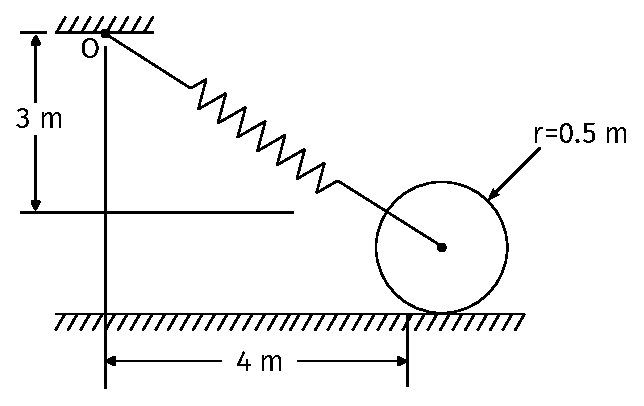
\includegraphics[width=0.9\textwidth,valign=c]{./figures/question7.eps}
%     \captionsetup{labelformat=empty}
%     \caption{\scriptsize DC motor drawing and schematic}
%     \label{fig:gear_system}
\end{minipage}
% \end{wrapfigure}


\end{questions}

\end{document}
